\documentclass[12pt]{article}

\usepackage{sbc-template}
\usepackage{graphicx,url}
\usepackage[utf8]{inputenc}
\usepackage[brazil]{babel}
\usepackage[table]{xcolor}
\usepackage{hyperref}
\sloppy

\title{Sistema Aberto de Gestão Universitário e Institucional}

\author{Ana Letícia O. Calandrine\inst{1}, Juan Carlos T. Martins\inst{1}, Yuri Gabriel C. Delgado\inst{1},\\
Ana Beatriz S. Serra\inst{1}, Anny Karoliny S. Costa\inst{1}, Marcely L. Anjos\inst{1},\\
Lucas S. Diniz\inst{1}, Henrique M. P. Silva\inst{1}, Juliana R. Pereira\inst{1},\\
João Davi C. Souza (Líder)\inst{1}, Woody M. Souza\inst{1}, Pedro Thiago B. Alves\inst{1},\\
Jamilly F. P. Correa\inst{1}, Heitor M. Versoza\inst{1}}

\address{Faculdade de Computação (FACOMP)\\
Instituto de Ciências Exatas e Naturais (ICEN)\\
Universidade Federal do Pará (UFPA)\\
Belém -- PA -- Brasil
\email{pessoa1@gmail.com, pessoa2@icen.ufpa.br, pessoa3@gmail.com,}\\
\vspace{-20px}
\email{pessoa4@tron.com}
}

\begin{document}

\maketitle

\begin{resumo}
O Sistema Aberto de Gestão Universitário e Institucional (SAGUI) consiste em uma plataforma educacional do tipo Learning Management System (LMS) concebida para centralizar a administração de cursos, disciplinas e materiais didáticos. Visando superar as restrições de ferramentas genéricas, a solução garante uma gestão refinada de ciclos de aprendizagem e operacionaliza regras de negócio acadêmicas de alta complexidade para três perfis de usuários: Administrador, Professor e Aluno. Este relatório consolida o trabalho integrado das equipes de desenvolvimento, documentando a arquitetura tecnológica global da aplicação. A infraestrutura de Back-End foi estabelecida como uma API RESTful em Java, empregando Spring Boot, banco de dados PostgreSQL e deploy via Docker, sendo estruturada em camadas lógicas e protegida por segurança baseada em JWT. Concomitantemente, o Front-End traduziu essas diretrizes em interfaces consistentes utilizando Next.js, TypeScript e Material UI (MUI), isolando a comunicação de rede por meio de uma arquitetura orientada a serviços. Em suma, o documento detalha as fundações sistêmicas e as implementações de módulos críticos que viabilizam este ecossistema educacional.

\end{resumo}

\textbf{Palavras-chave:} Sistema de Gestão da Aprendizagem, Arquitetura de Software, Sistema de Gestão Acadêmica, Next.js, Desenvolvimento Full-Stack.

\section{Introdução}

A contínua expansão das modalidades de ensino e o aumento na complexidade das normativas acadêmicas evidenciam as limitações de sistemas de gestão de aprendizagem (LMS) genéricos. Muitas dessas ferramentas carecem da flexibilidade necessária para orquestrar fluxos institucionais avançados, como etapas encadeadas de aprovação, progressão estruturada e um isolamento granular de privilégios. Para preencher essa lacuna tecnológica, desenvolveu-se o Sistema Aberto de Gestão Universitário e Institucional (SAGUI), entregando uma gestão rigorosa do progresso estudantil, separação clara de acessos e capacidade para processar regras educacionais personalizadas.

A operação do sistema é fundamentada em três perfis de acesso, cada um equipado com interfaces e fluxos exclusivos. O administrador detém controle global, gerenciando a criação de cursos, o deferimento de matrículas e a integridade cadastral (status ativo/inativo) no banco de dados. O professor foca na gestão pedagógica, possuindo autonomia para estruturar módulos, aulas e anexos unicamente dentro do escopo das disciplinas sob sua tutela. Por fim, o aluno atua como consumidor final da plataforma, acessando os catálogos e consumindo o conteúdo, submetido a trilhas de aprendizagem e critérios estritos de avaliação por desempenho.

Nesse contexto, o presente artigo tem como finalidade apresentar o trabalho consolidado de concepção, estruturação e implementação do SAGUI. Nas seções subsequentes, o relatório está organizado da seguinte forma: inicialmente, detalha-se a arquitetura tecnológica e estrutural do Front-End, incluindo sua camada própria de serviços, rotas e frentes de desenvolvimento de interface. Em seguida, será apresentada a arquitetura e a modelagem do Back-End, englobando o desenho da API, a persistência de dados e as lógicas de segurança da informação. Por fim, relatam-se as funcionalidades entregues de forma conjunta, validando o funcionamento integral do ecossistema.


\section{Arquitetura do Front-End}
A camada de front-end do SAGUI foi construída sobre o Next.js, utilizando o App Router, o que garante um roteamento robusto, a proteção de páginas por meio de middleware e uma performance otimizada para o lado do cliente. Sobre essa base, adotou-se o TypeScript como linguagem principal, assegurando tipagem estática e reduzindo drasticamente a ocorrência de erros em tempo de execução, o que contribui diretamente para a manutenibilidade do código ao longo do projeto. Para a camada visual, optou-se pela biblioteca de componentes Material UI (MUI), que impede estilizações arbitrárias e padroniza a interface do sistema, promovendo consistência entre as diferentes telas.

Como o desenvolvimento do front-end ocorreu em paralelo à evolução do back-end, adotou-se uma estratégia de integração baseada em funções assíncronas e na Context API do React para o gerenciamento do estado global da aplicação. Essa abordagem permitiu que as equipes avançassem na construção das telas mesmo antes da disponibilização completa da API, substituindo posteriormente os dados simulados por chamadas reais ao backend sem a necessidade de reescrever a lógica das páginas.

\subsection{Organização em Camadas da Aplicação}
Para evitar que as páginas React concentrassem responsabilidades que não lhes cabem, como chamadas HTTP, regras de negócio, tratamento de autenticação, validação de permissões e transformação de dados, a equipe estruturou uma camada própria de serviços e domínio da aplicação, análoga a uma camada de application/service layer. O código-fonte ficou dividido essencialmente em dois grandes diretórios: src/app, responsável pelas páginas, rotas, layouts e componentes de tela; e src/new-services, responsável pelas regras de negócio, pela comunicação com a API, pelos modelos de dados e pelo controle de acesso.

\newpage

\begin{figure}[htbp]
    \centering
    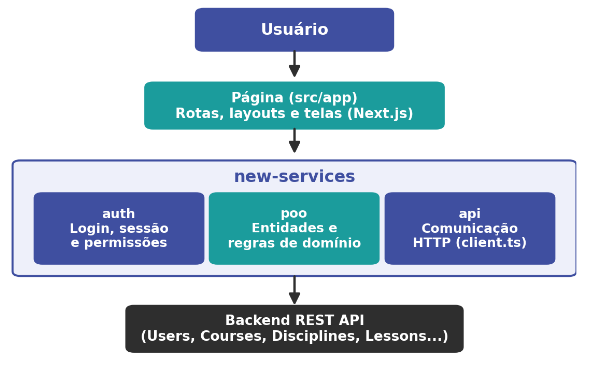
\includegraphics[width=0.7\textwidth]{imagem1.png}
    \caption{Arquitetura em camadas do Front-End}
    \label{fig:exemplo}
\end{figure}

A Figura 1 ilustra o fluxo entre essas camadas, desde a interação do usuário até o consumo da API REST do backend.

\begin{table}[htpb]
    \centering
    \label{tab:camadas_frontend}
    \renewcommand{\arraystretch}{1.5}
    \begin{tabular}{|l|l|}
    \hline
    \rowcolor[HTML]{229496} 
    \textbf{\textcolor{white}{Camada}} & \textbf{\textcolor{white}{Responsabilidade}} \\ \hline
    
    \textbf{app} & Rotas e páginas do sistema \\ \hline
    
    \rowcolor[HTML]{EFEFF5} 
    \textbf{components} & Interface visual reutilizável \\ \hline
    
    \textbf{contexts} & Estado global da aplicação \\ \hline
    
    \rowcolor[HTML]{EFEFF5} 
    \textbf{auth} & Login, sessão e controle de acesso \\ \hline
    
    \textbf{poo} & Regras de domínio das entidades \\ \hline
    
    \rowcolor[HTML]{EFEFF5} 
    \textbf{api} & Comunicação HTTP com o backend \\ \hline
    
    \textbf{types / requests / responses} & Modelos, payloads e retornos da API \\ \hline
    
    \rowcolor[HTML]{EFEFF5} 
    \textbf{cards} & Modelos de dados preparados para a UI \\ \hline

    \end{tabular}
    \caption{Camadas do Front-End}

\end{table}

A Tabela 1 sintetiza a responsabilidade de cada camada da aplicação front-end.

\subsection{Camada de Autenticação}
A pasta auth concentra tudo o que está relacionado ao usuário logado, incluindo login, cadastro, logout, recuperação do usuário autenticado, armazenamento de token e controle de permissões. A comunicação HTTP de autenticação fica isolada em um cliente dedicado, enquanto o contexto de autenticação mantém o estado global do usuário, transformando dados provenientes de localStorage, cookies e da própria API em informações prontamente utilizáveis pelas páginas, como o papel (role) do usuário logado. Complementarmente, um módulo de política de rotas define quais perfis podem acessar cada rota do sistema, e um módulo de validação de acesso executa essa checagem em tempo de navegação, bloqueando o carregamento de páginas para perfis não autorizados.

\nocite{*}

\bibliographystyle{sbc}
\bibliography{referencias}

\end{document}
